Nesse problema, consideramos o Hamiltoniano seguinte:

\begin{equation}
\hat{H} = \sum_{i \in \{ L,R \}} U \hat{n}_{i+} \hat{n}_{i-}
   - J \sum_{\sigma = \pm 1} ( c_{L\sigma}^{\dagger} c_{R\sigma}
   + c_{L\sigma}^{\dagger} c_{R\sigma}),
\end{equation}

onde $\hat{n}_{i\sigma} = c_{i\sigma}^{\dagger} c_{i\sigma}$. E temos as relações de anticomutação típicas de um sistema fermiônico:

\begin{subequations}
\begin{align}
\{ c_{i\sigma}^{\dagger},c_{j\sigma'}\}&=\delta_{i,j} \delta_{\sigma,\sigma'} \label{anti1} \\
\{ c_{i\sigma}^{\dagger},c_{j\sigma'}^{\dagger}\}&=0 \label{anti2} \\
\{ c_{i\sigma},c_{j\sigma'}\}&=0 \label{anti3}
\end{align}
\label{anti}
\end{subequations}

Calculamos agora as seguintes relações de comutação:

\begin{subequations}
\begin{align}
\left[ \hat{n}_{L+}, \hat{H} \right] &= -J \left(
c_{L+}^{\dagger} c_{R+} - c_{R+}^{\dagger} c_{L+} \right) \label{comm1} \\
\left[ \hat{n}_{R+}, \hat{H} \right] &= J \left(
c_{L+}^{\dagger} c_{R+} - c_{R+}^{\dagger} c_{L+} \right) \label{comm2} \\
\left[ \hat{n}_{L-}, \hat{H} \right] &= -J \left(
c_{L-}^{\dagger} c_{R-} - c_{R-}^{\dagger} c_{L-} \right) \label{comm3} \\
\left[ \hat{n}_{R-}, \hat{H} \right] &= J \left(
c_{L-}^{\dagger} c_{R-} - c_{R-}^{\dagger} c_{L-} \right) \label{comm4}
\end{align}
\label{comm}
\end{subequations}

Esses cálculos podem ser realizados com o auxílio das Equações \eqref{anti}. Chegamos portanto, se combinarmos \eqref{comm1} e \eqref{comm2}, a:

\begin{equation}
\left[ \hat{n}_{L+} + \hat{n}_{R+}, \hat{H} \right] = 0
\end{equation}

E, combinando \eqref{comm3} e \eqref{comm4}, chegamos a:

\begin{equation}
\left[ \hat{n}_{L-} + \hat{n}_{R-}, \hat{H} \right] = 0
\end{equation}

Portanto, os números de partículas de tipo $+$ e $-$ são quantidades conservadas. Isso nos permite restringir o problema a subespaços vetoriais específicos para achar o espectro de energia do sistema. Se definirmos o estado $\left|n_{+},i,n_{-},j \right> $ como o estado com $n_{+}$ partículas do tipo $+$ e $n_{-}$ partículas do tipo $-$, e com $i$ partículas do tipo $+$ no sítio $L$ e também $j$ partículas do tipo $+$ no sítio $L$. Teremos então, subespaços onde diagonalizar a matriz. Por exemplo, o subespaço constituído pelo vetor $\left| 2,1,2,1 \right>$ é um subespaço unidimensional, portanto é autovetor do Hamiltoniano. O subespaço constituído por $\left| 0,0,0,0 \right>$ também é outro unidimensional e, portanto, também autovetor do Hamiltoniano. Resta, então, analisar os subespaços de dimensão maior. Estes são os casos:

\begin{itemize}
\item[\textbf{A}] $\left| 1,0,0,0 \right>$ e $\left| 1,1,0,0 \right>$;
\item[\textbf{B}] $\left| 1,0,1,0 \right>$, $\left| 1,0,1,1 \right>$, $\left| 1,1,1,0 \right>$ e $\left| 1,1,1,1 \right>$;
\item[\textbf{C}] $\left| 1,1,2,1 \right>$ e $\left| 1,0,2,1 \right>$;
\end{itemize}

Teremos também, as reflexões $n_{+} \leftrightarrow n_{-}$. O que nos leva a outra simetria do problema. Essa simetria é a das reflexões $R \leftrightarrow L$. Como a inversão $R \leftrightarrow L$ é um operador cujo quadrado é a identidade, seus autovalores podem ser somente $\pm 1$. Portanto, precisamos de autoestados simétricos ou antisimétricos em relação a essa inversão. Para cada autoespaço acima, teremos os seguintes autovetores do operador $P$ responsável por $R \leftrightarrow L$:

\begin{itemize}
\item[\textbf{A}]
\begin{itemize}
\item[\textbf{.1}] $\frac{1}{\sqrt{2}}\left( \left| 1,0,0,0 \right> + \left| 1,1,0,0 \right> \right)$ ($P=+1$);
\item[\textbf{.2}] $\frac{1}{\sqrt{2}}\left( \left| 1,0,0,0 \right> - \left| 1,1,0,0 \right> \right)$ ($P=-1$);
\end{itemize}
\item[\textbf{B}]
\begin{itemize}
\item[\textbf{.1}] $\frac{1}{\sqrt{2}}\left( \left| 1,0,1,0 \right> + \left| 1,1,1,1 \right> \right)$ ($P=+1$);
\item[\textbf{.2}] $\frac{1}{\sqrt{2}}\left( \left| 1,0,1,0 \right> - \left| 1,1,1,1 \right> \right)$ ($P=-1$);
\item[\textbf{.3}] $\frac{1}{\sqrt{2}}\left( \left| 1,0,1,1 \right> + \left| 1,0,1,1 \right> \right)$ ($P=+1$);
\item[\textbf{.4}] $\frac{1}{\sqrt{2}}\left( \left| 1,0,1,1 \right> - \left| 1,0,1,1 \right> \right)$ ($P=-1$);
\end{itemize}
\item[\textbf{C}]
\begin{itemize}
\item[\textbf{.1}] $\frac{1}{\sqrt{2}}\left( \left| 1,0,2,1 \right> + \left| 1,1,2,1 \right> \right)$ ($P=+1$);
\item[\textbf{.2}] $\frac{1}{\sqrt{2}}\left( \left| 1,0,2,1 \right> - \left| 1,1,2,1 \right> \right)$ ($P=-1$);
\end{itemize}
\end{itemize}

Com mais uma cópia de \textbf{A} e outra do subespaço \textbf{C} temos vários subespaços já diagonalizados. Para fins de completeza, listamos todos abaixo, separados pela paridade $R \leftrightarrow L$:

\begin{itemize}
\item[\textbf{$n_{+} = 0$, $n_{-} = 0$}]
\begin{itemize}
\item[\textbf{.1}] $\left| 0,0,0,0 \right>$ ($P=+1$);
\end{itemize}

\item[\textbf{$n_{+} = 0$, $n_{-} = 1$}]
\begin{itemize}
\item[\textbf{.1}] $\frac{1}{\sqrt{2}}\left( \left| 0,0,1,0 \right> + \left| 0,0,1,1 \right> \right)$ ($P=+1$);
\item[\textbf{.2}] $\frac{1}{\sqrt{2}}\left( \left| 0,0,1,0 \right> - \left| 0,0,1,1 \right> \right)$ ($P=-1$);
\end{itemize}

\item[\textbf{$n_{+} = 0$, $n_{-} = 2$}]
\begin{itemize}
\item[\textbf{.1}] $\left| 0,0,2,1 \right>$ ($P=+1$);
\end{itemize}

\item[\textbf{$n_{+} = 1$, $n_{-} = 0$}]
\begin{itemize}
\item[\textbf{.1}] $\frac{1}{\sqrt{2}}\left( \left| 1,0,0,0 \right> + \left| 1,1,0,0 \right> \right)$ ($P=+1$);
\item[\textbf{.2}] $\frac{1}{\sqrt{2}}\left( \left| 1,0,0,0 \right> - \left| 1,1,0,0 \right> \right)$ ($P=-1$);
\end{itemize}

\item[\textbf{$n_{+} = 1$, $n_{-} = 1$}]
\begin{itemize}
\item[\textbf{.1}] $\frac{1}{\sqrt{2}}\left( \left| 1,0,1,0 \right> + \left| 1,1,1,1 \right> \right)$ ($P=+1$);
\item[\textbf{.2}] $\frac{1}{\sqrt{2}}\left( \left| 1,0,1,1 \right> + \left| 1,1,1,0 \right> \right)$ ($P=+1$);
\item[\textbf{.3}] $\frac{1}{\sqrt{2}}\left( \left| 1,0,1,0 \right> - \left| 1,1,1,1 \right> \right)$ ($P=-1$);
\item[\textbf{.4}] $\frac{1}{\sqrt{2}}\left( \left| 1,0,1,1 \right> - \left| 1,1,1,0 \right> \right)$ ($P=-1$);
\end{itemize}

\item[\textbf{$n_{+} = 1$, $n_{-} = 2$}]
\begin{itemize}
\item[\textbf{.1}] $\frac{1}{\sqrt{2}}\left( \left| 1,0,2,1 \right> + \left| 1,1,2,1 \right> \right)$ ($P=+1$);
\item[\textbf{.2}] $\frac{1}{\sqrt{2}}\left( \left| 1,0,2,1 \right> - \left| 1,1,2,1 \right> \right)$ ($P=-1$);
\end{itemize}

\item[\textbf{$n_{+} = 2$, $n_{-} = 0$}]
\begin{itemize}
\item[\textbf{.1}] $\left| 2,1,0,0 \right>$ ($P=+1$);
\end{itemize}

\item[\textbf{$n_{+} = 2$, $n_{-} = 1$}]
\begin{itemize}
\item[\textbf{.1}] $\frac{1}{\sqrt{2}}\left( \left| 2,1,1,0 \right> + \left| 2,1,1,1 \right> \right)$ ($P=+1$);
\item[\textbf{.2}] $\frac{1}{\sqrt{2}}\left( \left| 2,1,1,0 \right> - \left| 2,1,1,1 \right> \right)$ ($P=-1$);
\end{itemize}

\item[\textbf{$n_{+} = 2$, $n_{-} = 2$}]
\begin{itemize}
\item[\textbf{.1}] $\left| 2,1,2,1 \right>$ ($P=+1$);
\end{itemize}
\end{itemize}

Para diagonalizar completamente o Hamiltoniano, precisamos ainda lidar com o subespaço $\{ n_{+} = 1$, $n_{-} = 1 \}$, já que podemos combinar autoestados com a mesma paridade em relação à $L \leftrightarrow R$. Nesse subespaço, o Hamiltoniano toma a forma:

\begin{equation}
\begin{bmatrix}
U & 2J & 0 & 0 \\
2J & 0 & 0 & 0 \\
0 & 0 & U & 0 \\
0 & 0 & 0 & 0 \\
\end{bmatrix}
\end{equation}

Onde tomamos a base com os vetores da lista e na ordem em que aparecem na lista. Dessa forma, no subespaço $P=+1$(representado pelo bloco superior esquerdo da matriz) teremos as energias $E_{P=+1}=\frac{U\pm \sqrt{U^2+4J^2}}{2}$, e no outro subespaço($P=-1$), a matriz já está diagonal.
\par
O espectro de energia será, portanto:

\begin{itemize}

\item[$\{ n_{+} = 0$, $n_{-} = 0 \}$] $E=0$;

\item[$\{ n_{+} = 0$, $n_{-} = 1 \}$] 
\begin{itemize}
\item $E=-J$;
\item $E=+J$;
\end{itemize}

\item[$\{ n_{+} = 0$, $n_{-} = 2 \}$] $E=0$;

\item[$\{ n_{+} = 1$, $n_{-} = 0 \}$] 
\begin{itemize}
\item $E=-J$;
\item $E=+J$;
\end{itemize}

\item[$\{ n_{+} = 1$, $n_{-} = 1 \}$]
\begin{itemize}
\item $E=\frac{U+\sqrt{U^2+4J^2}}{2}$;
\item $E=\frac{U-\sqrt{U^2+4J^2}}{2}$;
\item $E=U$;
\item $E=0$;
\end{itemize}

\item[$\{ n_{+} = 1$, $n_{-} = 2 \}$] 
\begin{itemize}
\item $E=U-J$;
\item $E=U+J$;
\end{itemize}

\item[$\{ n_{+} = 2$, $n_{-} = 0 \}$] $E=0$;

\item[$\{ n_{+} = 2$, $n_{-} = 1 \}$] 
\begin{itemize}
\item $E=U-J$;
\item $E=U+J$;
\end{itemize}

\item[$\{ n_{+} = 2$, $n_{-} = 2 \}$] $E=2U$;

\end{itemize}

Podemos, agora, para cada número de partículas, calcular a função equipartição:

\begin{itemize}

\item[$\{ n_{+} = 0$, $n_{-} = 0 \}$] $Z=1$;

\item[$\{ n_{+} = 0$, $n_{-} = 1 \}$] $Z=2\cosh{\beta J}$;

\item[$\{ n_{+} = 0$, $n_{-} = 2 \}$] $Z=1$;

\item[$\{ n_{+} = 1$, $n_{-} = 0 \}$] $Z=2\cosh{\beta J}$;

\item[$\{ n_{+} = 1$, $n_{-} = 1 \}$] $Z=2e^{- \beta \frac{U}{2}}\left\{ \cosh{\beta \frac{U}{2}} + \cosh{\beta \frac{\sqrt{U^2+4J^2}}{2}} \right\}$;

\item[$\{ n_{+} = 1$, $n_{-} = 2 \}$] $Z=2e^{-\beta U} \cosh{\beta J}$;

\item[$\{ n_{+} = 2$, $n_{-} = 0 \}$] $Z=1$;

\item[$\{ n_{+} = 2$, $n_{-} = 1 \}$] $Z=2e^{- \beta U} \cosh{\beta J}$;

\item[$\{ n_{+} = 2$, $n_{-} = 2 \}$] $Z=e^{-2\beta U}$;

\end{itemize}

Daqui podemos tirar cinco funções equipartições distintas:

\begin{subequations}
\begin{align}
Z_1 &= 1 \\
Z_2 &= 2 \cosh{\left (J \beta \right )} \\
Z_3 &= 2 \left(\cosh{\left (\frac{U \beta}{2} \right )} + \cosh{\left (\frac{\beta \sqrt{4 J^{2} + U^{2}}}{2} \right )}\right) e^{- \frac{U \beta}{2}} \\
Z_4 &= 2 e^{- U \beta} \cosh{\left (J \beta \right )} \\
Z_5 &= e^{- 2 U \beta}
\end{align}
\label{equipart}
\end{subequations}

Podemos tirar os potenciais termodinâmicos dessas:

\begin{subequations}
\begin{align}
F_1 &= 0 \\
F_2 &= - \frac{\log{\left (2 \cosh{\left (J \beta \right )} \right )}}{\beta} \\
F_3 &= - \frac{- \frac{U \beta}{2} + \log{\left (\cosh{\left (\frac{U \beta}{2} \right )} + \cosh{\left (\frac{\beta \sqrt{4 J^{2} + U^{2}}}{2} \right )} \right )} + \log{\left (2 \right )}}{\beta} \\
F_4 &= U - \frac{\log{\left (2 \cosh{\left (J \beta \right )} \right )}}{\beta} \\
F_5 &= 2U
\end{align}
\end{subequations}

E também:

\begin{subequations}
\begin{align}
U_1 &= 0 \\
U_2 &= - J \tanh{\left (J \beta \right )} \\
U_3 &= - \frac{- U \left(\cosh{\left (\frac{U \beta}{2} \right )} + \cosh{\left (\frac{\beta \sqrt{4 J^{2} + U^{2}}}{2} \right )}\right) + U \sinh{\left (\frac{U \beta}{2} \right )} + \sqrt{4 J^{2} + U^{2}} \sinh{\left (\frac{\beta \sqrt{4 J^{2} + U^{2}}}{2} \right )}}{2 \cosh{\left (\frac{U \beta}{2} \right )} + 2 \cosh{\left (\frac{\beta \sqrt{4 J^{2} + U^{2}}}{2} \right )}} \\
U_4 &= - J \tanh{\left (J \beta \right )} + U \\
U_5 &= 2U
\end{align}
\end{subequations}

E, por fim:

\begin{subequations}
\begin{align}
S_1 &= 0 \\
S_2 &= J \beta \tanh{\left (J \beta \right )} - \log{\left (2 \cosh{\left (J \beta \right )} \right )} \\
S_3 &= \beta \left(\frac{\left(- \frac{U x_{2} \left(2 x_{3} + 2 x_{6}\right)}{2} + x_{2} \left(U \sinh{\left (x_{1} \right )} + x_{4} \sinh{\left (x_{5} \right )}\right)\right) e^{x_{1}}}{2 x_{7}} - \frac{\log{\left (2 x_{2} x_{7} \right )}}{\beta}\right) \\
S_4 &= J \beta \tanh{\left (J \beta \right )} - \log{\left (2 \cosh{\left (J \beta \right )} \right )} \\
S_5 &= 0
\end{align}
\end{subequations}

Onde definimos:

\begin{subequations}
\begin{align}
x_{0} &= \frac{\beta}{2} \\
x_{1} &= U x_{0} \\
x_{2} &= e^{- x_{1}} \\
x_{3} &= \cosh{\left (x_{1} \right )} \\
x_{4} &= \sqrt{4 J^{2} + U^{2}} \\
x_{5} &= x_{0} x_{4} \\
x_{6} &= \cosh{\left (x_{5} \right )} \\
x_{7} &= \quad x_{3} + x_{6}
\end{align}
\end{subequations}

Assim, temos todas as propriedades termodinâmicas do sistema determinadas analiticamente. Agora, introduzimos o \textit{grand canonical ensemble} para colocar o sistema em contato com um banho com potencial químico $\mu$. Dessa maneira, teremos a função equipartição do sistema fica:

\begin{equation}
Z = \sum_{N=0}^{4} z^N Z(N) \text{ onde: }
\begin{cases}
Z(N) & \text{ é a função para número de partículas igual a } N \\
z^N & \text{ é a fugacidade } e^{\beta \mu}
\end{cases}
\end{equation}

Podemos escrever as funções $Z(N)$ em termos das equações \eqref{equipart}. Explicitamente, elas ficam:

\begin{subequations}
\begin{align}
Z(0) &= 1 \\
Z(1) &= 4\cosh{\beta J} \\
Z(2) &= 2 + 2 + 2 \left(\cosh{\left (\frac{U \beta}{2} \right )} + \cosh{\left (\frac{\beta \sqrt{4 J^{2} + U^{2}}}{2} \right )}\right) e^{- \frac{U \beta}{2}} \\
Z(3) &= 4 e^{-\beta U} \cosh{\beta J} \\
Z(4) &= e^{-2\beta U} \\
\end{align}
\end{subequations}

Aplicando então a definição, podemos tirar daí a função equipartição do sistema, e dela todos os potenciais termodinâmicos. Em particular,podemos tirar $N$ o número médio de partículas no sistema. A definição é:

\begin{equation}
N = \frac{\partial \log(Z)}{\partial z}
\end{equation}

Podemos, da expressão de $N$, plotar seu comportamento em relação às variáveis termodinâmicas, em relação à $\beta$ e a $\mu$, podemos ver esse comportamento ilustrado na Figura \ref{N}. Os valores escolhidos de $U$ e $J$ foram pensados de maneira a aumentar a dependência do \textit{ground state} em relação à $\mu$. Para compreender melhor o comportamento observado a alto $\beta$. Que pode ser observado na Figura \ref{beta}.

\begin{figure}[!h]
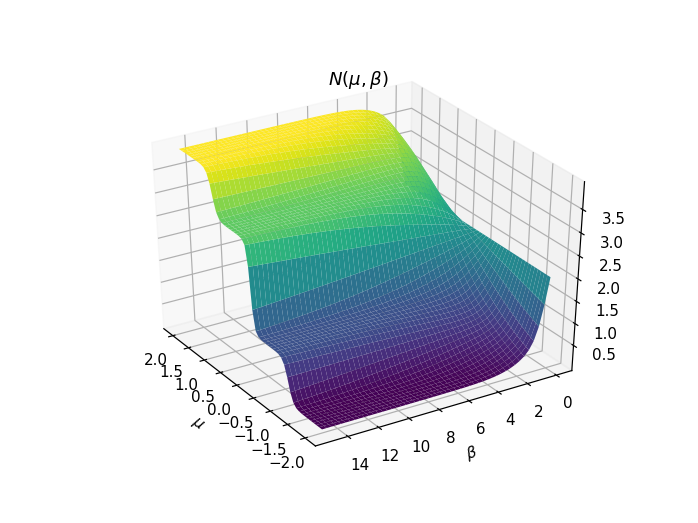
\includegraphics[scale=.5]{Content/N_mu_beta.png}
\caption{Comportamento de $\left<N\right>$ em relação a $\beta$ e $\mu$. Esolhemos os valores $U=0$ e $J=1$.}
\label{N}
\end{figure}

\begin{figure}[!h]
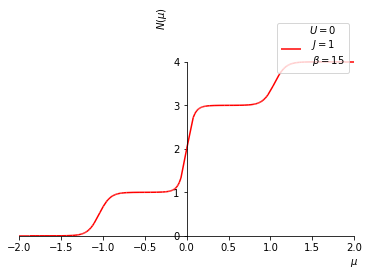
\includegraphics[scale=.7]{Content/N_mu.png}
\caption{Comportamento de $\left<N\right>$ em relação a $\mu$. Esolhemos os valores $U=0$, $\beta=15$ e $J=1$.}
\label{beta}
\end{figure}